\documentclass[a4paper]{article}
\usepackage{a4wide}
\usepackage[utf8]{inputenc}
\usepackage{amsmath}
\usepackage{mathtools}
\usepackage{amssymb}
\usepackage[english]{babel}
\usepackage{mdframed}
\usepackage{systeme,}
\usepackage{lipsum}
\usepackage{relsize}
\usepackage{caption}
\usepackage{tikz}
\usepackage{tikz-3dplot}
\usetikzlibrary{shapes.geometric}
\usepackage{pgfplots}
\usepackage{pgfplotstable}
\pgfplotsset{compat=newest}%1.7}
\usepackage{harpoon}%
\usepackage{graphicx}
\usepackage{wrapfig}
\usepackage{subcaption}
\usepackage{authblk}
\usepackage{float}
\usepackage{listings}
\usepackage{xcolor}
\usepackage{chngcntr}
\usepackage{amsthm}
\usepackage{comment}
\usepackage{commath}
\usepackage{hyperref}%Might remove, adds link to each reference
\usepackage{url}
\usepackage{calligra}

% Commands

\newcommand{\w}{\omega}
\newcommand{\curl}[1]{\mathbf{\nabla}\times \mathbf{#1}}
\newcommand{\grad}{\mathbf{\nabla}}
\newcommand{\dive}[1]{\mathbf{\nabla}\cdot \mathbf{#1}}
%\newcommand{\crr}{\mathfrak{r}}
\newcommand{\res}[2]{\text{Res}(#1,#2)}
\newcommand{\laplace}{\nabla^2}
\newcommand{\trace}{\text{Tr}}
\newcommand{\fpartial}[2]{\frac{\partial #1}{\partial #2}}
\newcommand{\rot}[3]{\begin{vmatrix}\hat{x}&\hat{y}&\hat{z}\\\partial_x&\partial_y&\partial_z\\#1&#2&#3 \end{vmatrix}}
\newcommand{\f}{\mathcal{F}}

% Special character commands
\DeclareMathAlphabet{\mathcalligra}{T1}{calligra}{m}{n}
\DeclareFontShape{T1}{calligra}{m}{n}{<->s*[2.2]callig15}{}
\newcommand{\crr}{\mathcalligra{r}\,}
\newcommand{\boldscriptr}{\pmb{\mathcalligra{r}}\,}



\title{Recap for FK7069}
\author{Author : Andreas Evensen}
\date{Date: \today}
\definecolor{codegreen}{rgb}{0,0.6,0}
\definecolor{codegray}{rgb}{0.5,0.5,0.5}
\definecolor{codepurple}{rgb}{0.58,0,0.82}
\definecolor{backcolour}{rgb}{0.95,0.95,0.92}

\lstdefinestyle{mystyle}{
    backgroundcolor=\color{backcolour},   
    commentstyle=\color{codegreen},
    keywordstyle=\color{magenta},
    numberstyle=\tiny\color{codegray},
    stringstyle=\color{codepurple},
    basicstyle=\ttfamily\footnotesize,
    breakatwhitespace=false,         
    breaklines=true,                 
    captionpos=b,                    
    keepspaces=true,                 
    numbers=left,                    
    numbersep=5pt,                  
    showspaces=false,                
    showstringspaces=false,
    showtabs=false,                  
    tabsize=2
}

\lstset{style=mystyle}

\begin{document}

\maketitle
\section{Introduction}
In this compendium I'll summarize the exercise made in the course, with the teachers solutions and dive into a recap of the content of the course.


\section{Introductory math}
In doing this compendium, I'll assume that the reader has a basic understanding of higher level mathematics. This includes the following topics: path-integrals, linear algebra, vector calculus, and differential systems.
This compendium will solve higher level physics problem and discuss solutions for modeling physical systems. The reader is also expected to have a basic understanding of the following topics: Classical mechanics, Electrodynamics, Quantum mechanics, and Statistical mechanics.
\subsection{Vector calculus}
In this section I'll give a brief recap of vector calculus. This is a very important tool in physics, and is used in almost all the exercises in this course.
\textit{Gradients} are used to describe the change in a function as a vector. Thus, the gradient takes a scalar function of two or more components and returns a vector-field.
\begin{align*}
    \grad f(x,y,z) &= \begin{pmatrix}\partial_x f(x,y,z)\\\partial_y f(x,y,z)\\\partial_z f(x,y,z)\end{pmatrix}.
\end{align*}We will use this to describe phenomena in \ref{sec: Soft matter} and \ref{sec: Fluid mechanics}. Divergence is also a very important tool in vector differential calculus.
It is used to describe the flux of a vector field through a surface. The divergence of a vector field is defined as:
\begin{align*}
    \dive{F} &= \partial_x F_x + \partial_y F_y + \partial_z F_z\\
    &= \begin{pmatrix}
        1\\
        1\\
        1\\
    \end{pmatrix}\cdot \begin{pmatrix}
        \partial_x F_x\\
        \partial_y F_y\\
        \partial_z F_z\\
    \end{pmatrix}.
\end{align*}Last but not least is the curl, which is the last type of vector differential calculus. The curl is used to describe the rotation of a vector field. The curl of a vector field is defined as:
\begin{align*}
    \curl{F} &= \begin{pmatrix}
        \partial_y F_z - \partial_z F_y\\
        \partial_z F_x - \partial_x F_z\\
        \partial_x F_y - \partial_y F_x\\
    \end{pmatrix}.
\end{align*}If a vector-field is conservative, the curl of that field, $\curl{F}$, is zero. Moreover, if a vector-field $u$ can be written as gradient of a scalar-field $\psi$, then:
\begin{align*}
    \curl{u} &= \curl{\grad \psi} = 0.
\end{align*}This implies that gradient fields are always conservative.
One thing to note is that this can be done in any generalized coordinate; however, in the scope of this course, we will only use Cartesian coordinates, Polar, and Spherical coordinates.
The definitions of such coordinate differentials can be found in any textbook on vector calculus.

\vspace{0.5cm}\noindent
There exist three types of integrals in vector-calculus: Path-integrals, surface-integrals, and volume-integrals. The path-integral is defined as:
\begin{align*}
    \int_{p} \mathbf{F}\cdot d\mathbf{r} &= \int_{p} F_x dx + F_y dy + F_z dz.
\end{align*}This is used to describe the work done by a force along a path. The surface-integral is defined as:
\begin{align*}
    \iint_{\mathcal{S}} \mathbf{F}\cdot d\mathbf{S} &= \iint_{\mathcal{S}} F_x dS_x + F_y dS_y + F_z dS_z.
\end{align*}This is used to describe the flux of a vector-field through a surface. The volume-integral is defined as:
\begin{align*}
    \iiint_{\mathcal{V}} \mathbf{F}\cdot d\mathbf{V} &= \iiint_{\mathcal{V}} F_x dV_x + F_y dV_y + F_z dV_z.
\end{align*}These integrals are often to complex to compute as is, and thus we use the following theorems: Green's theorem, Stokes' theorem, and the divergence theorem.
Greens theorem is used to convert a path-integral to a surface-integral. Stokes' theorem is used to convert a surface-integral to a path-integral. The divergence theorem is used to convert a volume-integral to a surface-integral.
The formulation of these theorems are as follows:
\begin{align*}
    \int_{\partial S} \mathbf{F}\cdot d\mathbf{r} &= \iint_{S} \curl{F}\cdot d\mathbf{S},\quad \text{Green's theorem}\\
    \iint_{S} \left(\curl{F}\right)\cdot d\mathbf{S} &= \oint_{\partial S} \mathbf{F}\cdot d\mathbf{r},\quad \text{Stokes' theorem}\\
    \iiint_{V} \left(\dive{F}\right)\cdot dV &= \iint_{\partial V} \mathbf{F}\cdot d\mathbf{S}\quad \text{Divergence theorem}.
\end{align*}These theorems are used to simplify the computation of integrals. One can therefore, almost always rewrite an integral to a simpler form, and thus compute the integral.
We will discuss two types of differential equations, namely: Ordinary differential equations (ODEs) and partial differential equations (PDEs). ODEs are differential equations that only depend on one variable, an example of this would be:
\begin{align*}
    \frac{d^2y}{dx^2} + \frac{dy}{dx} + y &= 0.
\end{align*}This is a second order ODE, and can be solved by using the characteristic equation. There exist multiple ways of solving ODEs, and we will not discuss further methods in this compendium, refer to any textbook on ODEs for further information, or visit \url{https://github.com/thesombady/FK7048/tree/main/Recap} which is a recap of the course FK7048, Mathematical methods.
Solving PDEs are quite a bit more complicated than solving ODEs, and we will discuss solutions later in the compendium. However, note that only a handful of PDEs can be solved analytically, and one often uses numerical solutions to solve PDEs; depending on the problem one utilizes different numerical methods: Finite difference methods, finite element methods, and so on.

\vspace{0.5cm}\noindent
All PDEs must have boundary at least $n$ boundary conditions if it's an $n$ dimensional problem, moreover, the solution must also have an initial condition; the initial condition simply states that the problem has an initial state.
The boundary conditions are used to describe how the solution behaves at the boundary of the problem; the boundary is dependent on the problem and can be a surface, a line or a volume, or higher dimensional objects.
There exist different types of boundary conditions, Dirichlet-, Neumann-, and Robin-boundary conditions are a few of them. They are written on the form of the following, in order:
\begin{align*}
    \psi &= \psi_0,\\
    \frac{\partial \psi}{\partial n} &= \psi_0,\\
    \frac{\partial \psi}{\partial n} &= \psi_0 + \alpha\psi.
\end{align*}At the different boundaries, the boundary conditions might be different, an example of this would be that a container is filled with a fluid, and that the fluid is being let out by a tap at the bottom.
The boundary condition at the top would be a Dirichlet boundary stating that the inlet of fluid is constant, and the other boundary condition would be a Neumann- or Robin-boundary condition, stating that the fluid is being let out at a rate proportional to the height of the fluid being build up in the container.

\vspace*{0.5cm}\noindent
There exist a few common PDEs that are used in physics, the most common ones are: The Laplace equation, the Poisson equation, the diffusion equation, the wave equation, and the heat equation.
\begin{align*}
    \laplace \psi &= 0,\\
    \laplace \psi &= f,\\
    \fpartial{\psi}{t} &= D\laplace \psi,\\
    \fpartial{\psi}{t} &= c^2\laplace \psi,\\
    \fpartial{\psi}{t} &= D\laplace \psi + f.
\end{align*}The Poisson equation is a generalization of the Laplace equation, and can be used in electrodynamics to describe the electric potential in a system. The solution for the Poisson equation is given by:
\begin{align*}
    \psi(\mathbf{r}) &= \frac{f}{\abs{\mathbf{r}}^2}.
\end{align*}This is a result we will use extensively, since the majority of PDEs can't be solved, one will try to rewrite it into something that is familiar.

\section{Soft Matter}\label{sec: Soft matter}
Suppose that one has an object that is 'soft', this means that when an external force is applied, that the object will deform.
\begin{figure}[H]
    \centering
    \begin{tikzpicture}[scale = 1.2]
        \draw (0,0) rectangle (4,3) node[right] {Object};
        \draw[fill = red] (2, 1) circle (1pt) node[above] {$\mathbf{P}$};
        \draw[fill = red] (2.5, 1.1) circle (1pt) node[above] {$\mathbf{P}'$};
        %\draw[->] (0, 0) -- (2, 1) node[midway, above] {$\mathbf{u}(\mathbf{P})$};
        \draw[->] (2, 1) -- (2.5, 1.1) node[right] {$\mathbf{u}(\mathbf{P}' - \mathbf{P})$};
        %\draw[->] (0, 0) -- (2.5, 1.1) node[midway, below] {$\mathbf{u}(\mathbf{P}')$};
    \end{tikzpicture}
    \caption{The deformation of a soft object.}
    \label{fig: soft object deformation derivation}
\end{figure}\noindent
The deformation field $u$ then describes how a point $\mathbf{P}$ moves under an external force $\mathbf{F}$. The deformation field $\mathbf{u}$ is only defined for small deformation, and by doing so it's a first order approximation of the actual deformation.
Taking the gradient of such a deformation field, one finds a second rank tensor-field, \textit{a matrix}, which then is the following:
\begin{align*}
    \grad{\mathbf{u}} &= \begin{pmatrix}
        \partial_x u_x & \partial_y u_x & \partial_z u_x\\
        \partial_x u_y & \partial_y u_y & \partial_z u_y\\
        \partial_x u_z & \partial_y u_z & \partial_z u_z\\
    \end{pmatrix}.
\end{align*}In two dimensions the dimension of the matrix is reduced from a $3\times 3$ to a $2\times 2$ matrix. Note that the gradient of $\mathbf{u}$ is actually the Jacobian of $\mathbf{u}$. If the deformation field $\mathbf{u}$ can be written as a gradient of a scalar field $\psi$, then the deformation field is conservative and the curl of the deformation field is zero.
This second rank tensor can then be decomposed in a symmetric and antisymmetric part:
\begin{align*}
    \grad{\mathbf{u}} &= \underbrace{\begin{pmatrix}
        \partial_x u_x &\frac{1}{2}\left(\partial_x u_y + \partial_y u_x\right) &\frac{1}{2}\left(\partial_xu_z + \partial_zu_x\right)\\
        \frac{1}{2}\left(\partial_y u_x + \partial_x u_y\right) & \partial_y u_y & \frac{1}{2}\left(\partial_zu_y + \partial_yu_z\right)\\
        \frac{1}{2}\left(\partial_zu_x + \partial_x u_z\right) & \frac{1}{2}\left(\partial_zu_y + \partial_yu_z\right) & \partial_z u_z\\        
    \end{pmatrix}}_{\text{Strain matrix}} \\
    &+ \underbrace{\begin{pmatrix}
        0 & \frac{1}{2}\left(\partial_xu_y - \partial_yu_x\right) & \frac{1}{2}\left(\partial_xu_z - \partial_zux\right)\\
        \frac{1}{2}\left(\partial_yu_x - \partial_xu_y\right) & 0 & \frac{1}{2}\left(\partial_yu_z - \partial_zu_y\right)\\
        \frac{1}{2}\left(\partial_zu_x - \partial_xu_z\right) & \frac{1}{2}\left(\partial_zu_y - \partial_yu_z\right) & 0\\
    \end{pmatrix}}_{\text{Rotation}}.
\end{align*}The strain matrix $s$ is symmetric, and the rotation matrix is antisymmetric. Using Einstein notation, one can write the individual components of the strain matrix as follows:
\begin{align*}
    s_{ij} &= \frac{1}{2}\left(\partial_i u_j + \partial_j u_i\right),\\
    s_{\alpha\beta} &= \frac{1}{2}\left(\partial_\alpha u_\beta + \partial_\beta u_\alpha\right).
\end{align*}If a volume element, in some coordinates of a body is given by $dX_1dX_2dX_3$, then the deformed volume element is given by $dX_1'dX_2'dX_3'$.
This can be expanded as $dX_1'dX_2'dX_3' = (1 + \lambda_1)dX_1(1 + \lambda_2)dX_2(1 + \lambda_3)dX_3$, where $\lambda_i$ is the eigenvalues of the strain matrix, where one has ignored the higher order terms.
This in itself is only valid if the deformation is small, and thus the higher order terms are negligible. The elements of the strain matrix that lies of the main diagonal are the elements that gives rise to a rotation, not a rotation transformation.

\vspace*{0.5cm}\noindent
Suppose a deformation field $\mathbf{u}(x,y) = a\left(0\hat{x} + x\hat{y}\right) = a\cdot\begin{pmatrix}0\\x\end{pmatrix}$, then the gradient matrix is given by:
\begin{align*}
    \grad{\mathbf{u}} &= \begin{pmatrix}
        \partial_x u_x & \partial_y u_x\\
        \partial_x u_y & \partial_y u_y\\
    \end{pmatrix} = a\cdot \begin{pmatrix}
        0 & 0\\
        1 & 0
    \end{pmatrix}.
\end{align*}The symmetric and antisymmetric parts are then given by:
\begin{align*}
    s &= \begin{pmatrix}
        0& \frac{a}{2}\\
        \frac{a}{2}&0
    \end{pmatrix},\\
    r &= \begin{pmatrix}
        0& -\frac{a}{2}\\
        \frac{a}{2}&0
    \end{pmatrix}.
\end{align*}The principal axis of the strain matrix is given by the eigenvectors of the strain matrix, and thus one finds the eigenvalues of the problem:
\begin{align*}
    \det\left(s - \lambda I\right) &= 0,\\
    \begin{vmatrix}
        -\lambda & \frac{a}{2}\\
        \frac{a}{2} & -\lambda
    \end{vmatrix} &= 0,\\
    \lambda^2 - \frac{a^2}{4} &= 0,\\
    \lambda &= \pm \frac{a}{2}.
\end{align*}The eigenvectors are then given by:
\begin{align*}
   s\cdot\mathbf{x_1} &= \lambda_1\mathbf{x_1},\\
   \implies x_1 &= \begin{pmatrix}
       1\\
       1
    \end{pmatrix},\\
    s\cdot\mathbf{x_2} &= \lambda_2\mathbf{x_2},\\
    \implies x_2 &= \begin{pmatrix}
        -1\\
        1
    \end{pmatrix}.
\end{align*}Now suppose another scenario, a body is being deformed by a deformation field $\mathbf{u}$. Its volume changed from $V$ to $V'$. Prove that the volume change is given by:
\begin{align*}
    \Delta V = \iint_{S}\mathbf{u}\cdot\hat{n}dS.
\end{align*}This change in volume $\Delta V$ is a result of the deformation field, and thus we can write the change in volume as:
\begin{align*}
    \Delta V &= \left(\dive{u}\right)\cdot V\\
    &= \iiint_{V} \left(\dive{u}\right)\cdot dV\\
    &= \iint_{\partial V}\mathbf{u}\cdot d\mathbf{S}
\end{align*}From this result, we can establish the following:
\begin{align*}
    \frac{\Delta V}{V} = \dive{u}.
\end{align*} This implies that the precentral change in volume is equal to the divergence of the deformation field.

\vspace*{0.5cm}\noindent
I've we then defined stress as being the symmetric part of the Jacobian of the deformation field, but what is then stress? 
Stress is also a second rank tensor, and is defined as the force per unit area. We start by saying that there are two 'solids' in contact with each other.
By Newtons third law, they exert a force on each other equal in size but opposite in direction. If we then say that the differential of the force, in one component is given by a linear relationship, we obtain the stress tensor:
\begin{align*}
    dF_i &= \sigma_{ij}dS_j,\\
    dF_i &= T_{i,j}dS_j
\end{align*}This $F$ is force per unit area, and to get the total force, one has to integrate over the entire surface, and by using the Divergence theorem, we can rewrite that integral as a volume integral instead:
\begin{align*}
    \mathbf{F} &= \iint_{\partial V}\mathbf{T}d\mathbf{S}\\
    &=\iiint_{V}\left(\dive{T}\right)dV.
\end{align*}Therefore, the force per unit area vector $\mathbf{f}$ is given by $\mathbf{f} = \dive{T}$. Generally, the divergence of a vector field is a scalar quantity, however, in this case it's actually a vector quantity.
If one combines what we know so far about stress with the equations of motion, one obtains the following expression:
\begin{align*}
    \rho\frac{d v_i}{dt} &=\partial_jT_{ij},\\
    \rho\frac{dv_\alpha}{dt} &= \partial_\beta\sigma_{\alpha\beta}.
\end{align*}The difference between the normal equations of motion is that we only have mass density $\rho(x,y,z)$ instead of mass; we look at all individual points within the body.
Within most cases, however, the problem is static, i.e. that the body does not move, but only gets deformed, and thus the equations of motions simply becomes:
\begin{align*}
    \partial_jT_{ij} &= 0,\\
    \partial_\beta\sigma_{\alpha\beta} &= 0.
\end{align*}We have so far assumed that the forces are localized interactions between the molecules of the body; this is a valid assumption in most cases due to the majority of matter being neutrally charged; hence, the forces keeping the body together are dipole-interactions which has short radii.
However, if the body is constructed of charged material, then this approach does not work. Generally, the stress tensor obeys at the boundary:
\begin{align*}
    \sigma_{\alpha\beta}n_\beta &= 0,\\
    T_{i,j}n_j &= 0,
\end{align*}which simply means that the stress tensor is perpendicular to the surface of the body. This is a result of force-balancing; torque-balancing also plays a role, which shows that the stress tensor is symmetric; just like the strain tensor.
In the stress tensor, we have two indices, these two are the directions of the stress in the object. The first index is the direction of the second index, which then is the boundary. So at $x$ we have directions in the $x$ direction and in the $y$ direction which then yields the elements of $T$ to be written as:
\begin{align*}
    T_{xx} &= \sigma_{xx},\quad \text{$x$ direction}\\
    T_{yx} &= \sigma_{yx}\quad \text{$y$ direction}.
\end{align*}Suppose that a 'soft' body has an external force $\mathbf{P}$ acting on its surface; if the body is in equilibrium, then show that the average stress, defined as:
\begin{align*}
    \langle\sigma_{\alpha\beta}\rangle &=\frac{1}{V}\int_V \sigma_{\alpha\beta}dV,
\end{align*}is given by:
\begin{align*}
    \langle\sigma_{\alpha\beta}\rangle &= \frac{1}{2V}\oint P_\alpha x_\beta + P_\beta x_\alpha dS.
\end{align*}First, we can define the stress tensor as:
\begin{align*}
  \sigma_{\alpha\beta} &= \frac{1}{2}\left(\frac{\partial T_{\alpha\beta}}{\partial x_\gamma} x_\gamma + T_{\gamma\beta}\delta_{\alpha\gamma}\right),
\end{align*}where $T_{\alpha\beta}$is the Cauchy stress tensor, and $\delta_{\alpha\beta}$ is the Kronecker delta. Now, we can use the divergence theorem to write:
\begin{align*}
  \oint \mathbf{T} \cdot \mathbf{n} dS &= \int_V \nabla \cdot \mathbf{T} dV,
\end{align*}where n is the outward-pointing normal vector to the surface. The Cauchy stress tensor can be decomposed into the stress tensor and the body force:
\begin{align*}
  \mathbf{T} &= \mathbf{\sigma} + \mathbf{P},
\end{align*}where P is the body force vector. Using these definitions, we can write:
\begin{align*}
  \oint (\mathbf{\sigma} + \mathbf{P}) \cdot \mathbf{n} dS &= \int_V \nabla \cdot \mathbf{\sigma} + \nabla \cdot \mathbf{P} dV.
\end{align*}Since the body is in equilibrium, $\dive{P}=0$. Then, using the definition of the average stress, we can write:
\begin{align*}
  \oint \sigma_{\alpha\beta} x_\beta + P_\alpha \cdot \mathbf{n} dS &= \int_V \frac{\partial \sigma_{\alpha\beta}}{\partial x_\gamma} x_\gamma dV.
\end{align*}Integrating both sides of the equation, we get:
\begin{align*}
  \frac{1}{2}\oint P_\alpha x_\beta + P_\beta x_\alpha dS &= \langle\sigma_{\alpha\beta}\rangle.
\end{align*}Thus, the average stress is given by:
\begin{align*}
  \langle\sigma_{\alpha\beta}\rangle &= \frac{1}{V}\int_V \sigma_{\alpha\beta}dV.
\end{align*}

\vspace*{0.5cm}\noindent
Elasticity and energy is also a great concept within soft matter. Suppose that when a body is deformed, it requires some work to obtain the new state; the change in work is then given by:
\begin{align*}
    \delta W = -\sigma_{\alpha\beta}\delta s_{\alpha\beta},
\end{align*}where $\sigma$ is the stress tensor and $\delta s$ is the strain tensor. Using the definition of the Helmholtz free energy, we state:
\begin{align*}
    TdS &= dU - \sigma_{\alpha\beta}d s_{\alpha\beta},
\end{align*}where $T$ is the temperature, $S$ is the entropy and $U$ is the stored energy; we use the stored energy as the free energy.
How does one then obtain the free energy $\f$? One can use Landau theory to obtain the free energy. This leads to the following expression:
\begin{align}
    \f = \f_0 + \frac{1}{2}\lambda s_{\alpha\alpha}^2 + \mu s_{\alpha\beta}s_{\alpha\beta},\label{eq: free energy lame coefficients}
\end{align}where $\f_0$ is trivially set to $0$. $\lambda$ and $\mu$ are the so called Lamé coefficients.
The strain tensor $s_{\alpha\beta}$ can be decomposed into two separate tensors, the pure sheer and volume change strain tensor. 
\begin{align*}
    s_{\alpha\beta} &= \underbrace{\left(s_{\alpha\beta} - \frac{1}{3}\delta_{\alpha\beta}s_{\nu\nu}\right)}_{\text{Pure sheer}} + \underbrace{\frac{1}{3}\delta_{\alpha\beta}s_{\nu\nu}}_{\text{Volume}}.
\end{align*}Using this decomposition of the strain tensor, one can rewrite the free energy eq\eqref{eq: free energy lame coefficients} as:
\begin{align*}
    \f &= \mu\left(s_{\alpha\beta} - \frac{1}{3}\delta_{\alpha\beta}s_{\nu\nu}\right)^2 + \frac{1}{2}K\frac{1}{3}\delta_{\alpha\beta}s_{\nu\nu}^2,
\end{align*}where $\mu$ is the so-called sheer modulus and $K$ is the bulk modulus of the material, $K = \lambda + \frac{1}{3}\mu$.

\vspace*{0.5cm}\noindent
What is then elasticity, or Elastostatics? It's the study of how soft body can deform under an external force.
We do elastostatics by the means of Navier-Cauchy equations; which is a set of PDEs that describes the motion of a soft body under some deformation.
\begin{align}
    \left(\lambda + \mu\right)\mathbf{\nabla}\left(\dive{u}\right)+\mu\laplace{u} &=0, \label{eq: Navier-Cauchy}
\end{align}This however can be rewritten with the Young's modulus $Y$ and the Poisson ratio $\sigma$; we have some bad naming convention here since $\sigma$ is also the stress.
\begin{align*}
    Y = \frac{9K\mu}{3K + \mu}, \quad \sigma = \frac{1}{2}\left(\frac{3K - 2\mu}{3K + \mu}\right).
\end{align*}The equations of elasticity can then be written as:
\begin{align*}
    \f &= \frac{Y}{2(1 + \sigma)}\left(s_{\alpha\beta}^2+ \frac{\sigma}{1-2\sigma}s_{\nu\nu}^2\right),\\
    \sigma_{\alpha\beta}&= \frac{Y}{1+\sigma}\left(s_{\alpha\beta} + \frac{\sigma}{1-2\sigma}\delta_{\alpha\beta}s_{\nu\nu}\right),\\
    \implies -\frac{2(1+\sigma)}{Y}\mathbf{f} &= \frac{1}{1-2\sigma}\nabla\left(\dive{u}\right) + \nabla^2\mathbf{u}.
\end{align*}Here, $\mathbf{f}$ is then the external force per unit volume. If the external force is $0$, then the equation of elasticity becomes easier, and can be computed with numerous methods, one of them being the Fourier transform and the Green's function.
One can also use numerical methods to solve the PDE as is. The homogenous equation of elasticity, given by eq \eqref{eq: Navier-Cauchy}, can also be written with the Poisson ratio $\sigma$ instead of the Lamé coefficients $\lambda$ and $\mu$;
\begin{align}
    \nabla\left(\dive{u}\right)+(1-2\sigma)\laplace{u} &= 0. \label{eq: Hom Navier-Cauchy Poisson}
\end{align}The homogenous equation of elasticity is very nice in the sense that is a second order linear PDE, and therefore the PDE exhibits certain properties.
Mainly, that there exists a unique solution to the problem and superposition of solutions, and that the symmetry of the problem is reflected in the symmetry of the solution, e.g. if the system is spherically symmetric, the solution is going to be spherically symmetric.

\vspace*{0.5cm}\noindent
In balancing the external force and the internal force, we reach the following:
\begin{align*}
    \sigma_{\alpha\beta}n_\beta = f_\alpha^{\text{surf}},
\end{align*}where $f^{\text{surf}}$ is the force per unit area. We can use this fact to derive the boundary conditions when to bodies are place in contact with each other; this could for example be when we fix a soft body against a rigid one.
At the interface between the two medium, thus we assume a cylindrical volume element;
\begin{figure}[H]
    \centering
    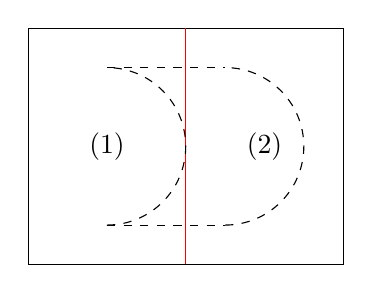
\begin{tikzpicture}
        \draw[] (0,0) rectangle (2, 3);
        \draw[] (2,0) rectangle (4, 3);
        \node at (1, 1.5) {$(1)$};
        \node at (3, 1.5) {$(2)$};
        \draw[color = red] (2,0) -- (2,3);
        \draw[dashed] (2.5, 0.5) arc (-90:90:1);
        \draw[dashed] (1, 0.5) arc (-90:90:1);
        \draw[dashed] (1, 0.5) -- (2.5, 0.5);
        \draw[dashed] (1, 0.5 + 2) -- (2.5, 0.5 + 2);
    \end{tikzpicture}
    \caption{A cylindrical volume element.}
    \label{fig: cylindrical volume element}
\end{figure}\noindent
The area encapsulated in the cylinder at the interfaces is then $\Delta S$, balancing the momentum one gets:
\begin{align*}
    \int_V \partial_\beta\sigma_{\alpha\beta}dV &= \int_V f_\alpha^\text{volume}dV,\\
    \implies \left(\sigma_{\alpha\beta}^{(1)} - \sigma_{\alpha\beta}^{(2)}\right)n_\beta &= f_\alpha^\text{surf}.
\end{align*}The superscript $(1)$ and $(2)$ denotes the two different bodies. Only if the surface force between the two bodies, is the stress tensor continuous across the boarder, otherwise, the stress tensor has a discontinuity. This can be seen when two objects are in contact with each other, and they do not mix.

\vspace{0.5cm}\noindent
Assume two spheres in contact with each other; both having some radii $R_1$ and $R_2$, and Young's modulus $Y_1$ and $Y_2$. The spheres are then pushed together with a force $F$ and are compressed a distance $h$.
\begin{figure}[H]
    \centering
    \begin{tikzpicture}
        \draw (0,0) circle (2cm);
        \draw (3.8,0) circle (2cm);
        \draw[<->, color = blue] (1.8, 0) -- (2, 0) node[below, pos = 0.5] {$h$};
    \end{tikzpicture}
    \caption{Figure of the system}
    \label{fig: hertzian spheres}
\end{figure}\noindent The contact area between the two sphere is a circle with radius $a$. Using this, one can estimate the displacement $h$\footnote{\url{https://en.wikipedia.org/wiki/Contact_mechanics}}:
\begin{align*}
    h&\propto \frac{F^{\frac{2}{3}}}{\left(Y_h\cdot R_H\right)^{\frac{2}{3}}},\\
    R_H &= \frac{1}{R_1} + \frac{1}{R_2}, \quad Y_H = \frac{1}{Y_1} + \frac{1}{Y_2},\\
    a&\propto \left(\frac{R_H\cdot F}{Y_H}\right)^{\frac{1}{3}}.
\end{align*}

\subsection{Plates and bending}
Assume we have a plate, which is being bent. The plate has some thickness and being bent by some external force.
\begin{figure}[H]
    \centering
    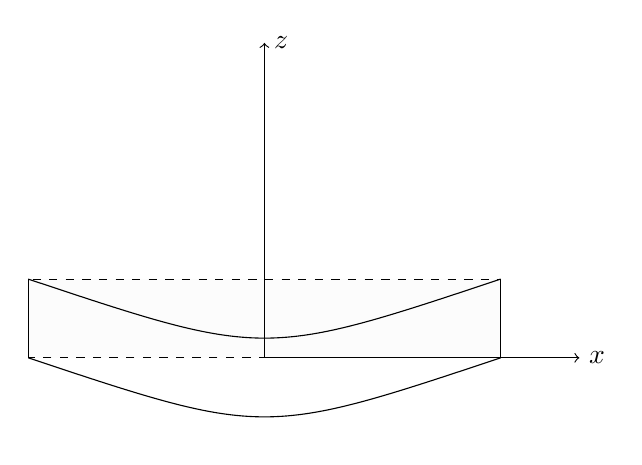
\begin{tikzpicture}
        \draw[dashed, fill = gray!2] (-3, 0) rectangle (3, 1);
        \draw[->] (0, 0) -- (4, 0) node[right] {$x$};
        \draw[->] (0, 0) -- (0, 4) node[right] {$z$};
        %\draw[->] (0, 0) -- (-1, -1) node[right] {$y$};
        \draw (-3, 0) .. controls (0, -1) .. (3, 0);
        \draw (-3, 1) .. controls (0, 0) .. (3, 1);
        \draw (-3, 0) -- (-3, 1);
        \draw (3, 0) -- (3, 1);
    \end{tikzpicture}
    \caption{Bent plate in the $xy$ plane}
    \label{fig: bent plate}
\end{figure}\noindent
One has that $\sigma_{xz} = \sigma_{yz} = \sigma_{zz} = 0$, which is on all the surfaces, but also that the deformation is only a function of $x$ and $y$, and thus $u_z^{(0)} = w(x,y)$.
\begin{align*}
    \sigma_{zx} &= \frac{Y}{1+\sigma}s_{zx}\\
    \sigma_{zy} &= \frac{Y}{1+\sigma}s_{zy}\\
    \sigma_{zz} &= \frac{Y}{(1+\sigma)(1-2\sigma)}\left(\left[1-\sigma\right]s_{zz} + \sigma\left[s_{xx} + s_{yy}\right]\right)\\
    \implies \frac{\partial u_x}{\partial z} &= - \frac{\partial u_z}{\partial x}\&\quad \frac{\partial u_y}{\partial z} = - \frac{\partial u_z}{\partial y}\quad\quad\quad (*)\\
    s_{zz} &= -\frac{\sigma}{1-\sigma}\left(s_{xx} + s_{y}\right)
\end{align*}The equation $(*)$ can be expressed with $w(x,y)$ instead, since the $u$ is the displacement in the $z$ direction. Thus, $u_x = -z\cdot \partial_x w(x,y)$ and $u_y = -z\cdot\partial_y w(x,y)$.
The strain tensor $s$ can thus be expressed with our variables $u$:
\begin{align*}
    s_{xx} &= -z \frac{\partial^2 w(x,y)}{\partial x^2} \quad \& \quad s_{yy} = -z \frac{\partial^2 w(x,y)}{\partial y^2},\\
    s_{xy} &= s_{yx} = -z \frac{\partial^2 w(x,y)}{\partial x\partial y},\\
    s_{zz} &= -\frac{\sigma}{1-\sigma}\left(s_{xx} + s_{y}\right)\\
    &=\frac{\sigma\cdot z}{1 - \sigma}\left(\nabla^2 w(x,y)\right).
\end{align*}The free energy $\f$ is then given by:
\begin{align*}
    \f &= \int_V F(x,y,z)dxdydz\\
    &=\int_V \underbrace{\frac{Y}{2(1 + \sigma)}\left(s_{\alpha\beta} + \frac{\sigma}{1 - 2\sigma}\delta_{\alpha\beta}s_{\nu\nu}\right)}_{F(x,y,z)}dxdydz\\
    &=\int_{-\frac{h}{2}}^\frac{h}{2} dz \left(z^2\right) \iint \frac{Y}{2(1 + \sigma)}\left(s_{\alpha\beta} + \frac{\sigma}{1 - 2\sigma}\delta_{\alpha\beta}s_{\nu\nu}\right)dxdy\\
    &=\frac{Yh^3}{24(1 - \sigma^2)}\underbrace{\iint \left(\left[\nabla^2w\right]^2 + 2(1-\sigma)\left[\left(\frac{\partial^2 w}{\partial x\partial y}\right)^2 - \frac{\partial^2 w}{\partial x^2} \frac{\partial^2 w}{\partial y^2}\right]\right)dxdy}_{\f_{\text{plate}}}
\end{align*}
Moreover, since the plates free energy is a function of $w(x,y)$, which is the displacement in the $z$ direction, we can often estimate the $w(x,y)$ function by a curvature. Therefore, the free energy of the plate can be written as:
\begin{align*}
    \f_{\text{2d}}^{\text{plate}} &= B\int_{\partial V} \left(\frac{1}{R_1} + \frac{1}{R_2}\right)^2dx_1dx_2
\end{align*}where then $B$ is the so-called bending modulus, and $R_1$ and $R_2$ are the radii of curvature of the plate. The bending modulus is given by:
\begin{align*}
    B &= \frac{Yh^3}{24(1-\sigma^2)}\quad \text{By comparison from above expression}
\end{align*}The bending modulus is a measure of how stiff the plate is, and is a measure of how much energy is required to bend the plate. The bending modulus is a measure of the stiffness of the plate, and is a measure of how much energy is required to bend the plate.

\vspace*{.5cm}\noindent
One can divide the phenomena in two cases, bending with stretching and bending without stretching. If one has without stretching, one can use a cylindrical system, whilst with stretching, one has to divide the system up in to components.
\begin{align*}
    \f_{2d}^{BS} &= \underbrace{B\int_{\partial V}\left(\frac{\partial^2}{\partial x^2} + \frac{\partial^2}{\partial x^2}\right)w\cdot dxdy}_{\text{Bending free energy}} + \underbrace{\frac{Y_{\text{2d}}}{2(1+\sigma_{\text{2d}})}\int_{\partial V}\left(s_{\alpha\beta}^2 + \frac{\sigma_{\text{2d}}}{1-\sigma_{\text{2d}}}\delta_{\alpha\beta}s_{\nu\nu}\right)dxdy}_{\text{Stretching free energy}}
\end{align*}
An example of this would be the following: the bending and stretching of a plate being pressed down.
\begin{figure}[H]
    \centering
    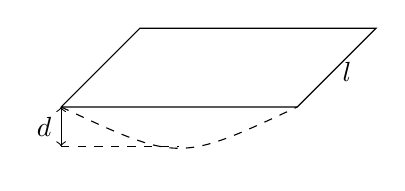
\begin{tikzpicture}
        \draw (0,0) -- (3,0) -- (4, 1) node[right, pos = 0.45] {$l$} -- (1, 1) -- (0, 0);
        %\draw[dashed] (0,0 - 0.5) -- (3,0 - 0.5) -- (4, 1 - 0.5) -- (1, 1 - 0.5) -- (0, 0 - 0.5);
        \draw[<->] (0, 0) -- (0, -0.5) node[left, pos = 0.5] {$d$};
        \draw[dashed] (0, 0) .. controls (1.5, -.7) .. (3, 0);
        \draw[dashed] (0, -.5) -- (1.5, -.5);
    \end{tikzpicture}
    \label{fig: plate bending}
    \caption{Figure of the system}
\end{figure}\noindent
The Young's modulus $Y_{\text{2d}}$ and the Bending modulus $B$ are given by:
\begin{align*}
    Y_{\text{2d}} &= \frac{Yh}{1-\sigma^2},\\
    B &= \frac{Yh^3}{24(1-\sigma^2)}.
\end{align*}The displacement $d$ is almost $w(x,y)$ and since we're in the order of $l$ of length scale, $\partial w$ is of the order $\frac{d}{l}$.
Therefore,
\begin{align*}
    \frac{\partial w}{\partial x_1}\frac{\partial w}{\partial x_2} \approx \left(\frac{d}{l}\right)^2\quad\&\quad \frac{\partial^2 w}{\partial x_\alpha} \approx \frac{d}{l^2}.
\end{align*}The stretching and bending contributes in the order of:
\begin{align*}
    \frac{Y_{\text{2d}}d^4}{l^4}l^2 \quad &\& \quad \frac{Bd^2}{l^4}l^2,\\
    \implies \frac{\frac{Y_{\text{2d}}d^4}{l^4}l^2}{\frac{Bd^2}{l^4}l^2} &=\frac{Y_{\text{2d}}d^2}{B}= \left(\frac{d}{h}\right)^2.
\end{align*}If the sheet is very thin, i.e. $d >> h$ then the stretching is greater than the bending, and otherwise vice-versa.
Thus, if one pushes down on the sheet, the sheet will deform with a circular curvature, say with radii $a$.
The area is then proportional to $a^2$ and the work done is simply the $f^{\text{surf}}\cdot d\sim Y_{\text{2d}}\left(\frac{d}{l}\right)^4$. This comes from the stretching of the sheet.
Therefore, the displacement $d$ is proportional to $\left(f^{\text{surf}}\right)^\frac{1}{3}$.

\subsection{Shells}
When dealing with shells, the strain has another contribution, namely the curvature of the shell. Thus, the strain tensor is given by:
\begin{align*}
    s_{\alpha\beta} &= \frac{1}{2}\left(\partial_\alpha u_\beta + \partial_\beta u_\alpha\right) + \frac{\partial w}{\partial x_\alpha}\frac{\partial w}{\partial x_\beta} + \delta_{\alpha\beta}\left(\frac{w}{R}\right),
\end{align*}here $R$ is the radii of curvature, and in the case of a flat plane, $R \to\infty$ and thus the last term vanishes.
The quantity $\f_{\text{Stretch}}/\f_{\text{Bend}}$ is then the so called Föpl-VonKarman number, FVK for short, which typically is of the order $R^2/h^2$, where $h$ is the thickness of the plate.
\subsection{Polymer}
A polymer is a long chain of monomers, which are connected by chemical bonds. The monomers are typically small molecules, however, they can also be larger molecules.
\begin{figure}[H]
   \centering
   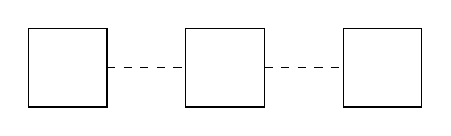
\begin{tikzpicture}
        \draw (0,0) rectangle (1,1);
        \draw[dashed] (1, 0.5) -- (2, 0.5);
        \draw (2,0) rectangle (3,1);
        \draw[dashed] (3, 0.5) -- (4, 0.5);
        \draw (4,0) rectangle (5,1);
   \end{tikzpicture} 
   \caption{A polymer example}
   \label{fig: polymer example}
\end{figure}\noindent
The polymer is therefore, typically, a long chain of monomers, which can be oriented differently. A polymer can therefore have a curvature.
This curvature, however, is a result of bending the chain, and this bending is costly; the cost lies in changing the bond-angle. The bond-angle is the angle between the monomers.
Typically, the bond-angle is determined by the type of chemical bond, and thus changing the bond-angle increases the free energy of the system.

\vspace*{0.5cm}\noindent
The bending energy is however typically small compared to that of the thermal energy of the polymer, which is in order of $k_bT$.
There exists some typical questions regarding polymers a physicist can ask: What is the average length of the polymer, What is the force required to pull the polymer a distance $d$, ... .
If one has a polymer, fastened at one end, which is straight but being deformed by some bending, then the free energy is given by:
\begin{align*}
    \f^{\text{bend}} &= \frac{B}{2}\int_0^L \frac{1}{R^2} ds\\
    &=\frac{BL}{2R^2},
\end{align*}if the polymer is bent in only a small bit, one can substitute $L = R\theta$, where $\theta$ is the angle of the bend, which leads to the following:
\begin{align*}
    \f^{\text{bend}} &=\frac{BL\theta^2}{2L^2}\\
    &= \frac{B\theta^2}{2L}\sim k_bT.
\end{align*}From this, one finds that there exists a characteristic length scale of the polymer: $L\sim \frac{B}{k_bT}$. One calls this length scale the persistence length $\mathcal{S}_p = \frac{B}{k_bT}$.
Now suppose a polymer which has a length $L$, which is much greater than the persistence length $\mathcal{S}_p$. The polymer is then in a random coil configuration; and can be described by a random walk; if the length of the polymer is much less than the persistence length, then the polymer is in a rod-like configuration, i.e. mostly straight.

\vspace*{0.5cm}\noindent
\begin{figure}[H]
    \centering
    \begin{tikzpicture}
        \begin{axis}[
            axis lines = left,
            xlabel = $x$,
            ylabel = $y$,
        ]
           \addplot[domain = 0:3, samples = 50, mark = -, mark options = {solid}] {2*x + 0.1*x^2 + 20 * ln(x) + 0.8 * x^3} node[below, pos = 0.7] {$\hat{t}$};

        \end{axis}
    \end{tikzpicture}
    \label{fig: polymer worm model}
    \caption{Path integral from polymer worm model}
\end{figure}\noindent
The bending energy is thus defined by the following:
\begin{align*}
    \f^{\text{bend}} &= \frac{B}{2}\int_0^L \left(\frac{1}{R}\right)^2ds\\
    &= \frac{B}{2}\int_0^L \left(\frac{d\hat{t}}{ds}\right)^2ds,\\
\end{align*}where $\hat{t}(s)$ then traces the entire path of the polymer. We like to draw the concepts to that of statistical physics, but for that we need to find the partition function $Z$, which is not an easy task.
The partition function is a functional of $\hat{t}(s)$, which thus implies:
\begin{align*}
    Z[\hat{t}] &= \sum_{\hat{t}_i(s)} \exp\left(-\frac{1}{k_bT}\cdot\left[\text{energy of }\hat{t}(s)\right]\right).
\end{align*}This is then expanded by discretizing the path $\hat{t}(s)$ with $N$ points, which yields:
\begin{align*}
    Z[\hat{t}] &=\int \Delta\hat{t}(s)\exp\left[-\frac{\mathcal{S}_p}{2}\int_0^L\left(\frac{d\hat{t}}{ds}\right)^2ds\right].
\end{align*}We really want to obtain the partition function, since $\f = k_bT\ln(Z)$, however this is still quite a difficult task.
If we restrict ourselves to one dimension, and state that there is no cost in bending; then we can safely assume that the polymer will exhibit random walk properties.
If the polymer is constructed of monomers of length $l$, then the average square length of the random walk of $N$ steps is given by: $\langle l^2\rangle = N \cdot a^2$.

\vspace*{0.5cm}\noindent
Helmholtz free energy is then given by:
\begin{align*}
    \f &= U - TS = -TS,
\end{align*}since there is no internal energy in the system, the entry however, can be rewritten as $S = k_b\cdot \ln(W)$ where $W$ is the number of microstates/all possible configurations.
One question still remains, what is the average length $l$ of the random walk? We can say that after $N$ steps, that we have stepped $M$ steps in one direction, and $N-M$ steps in the other direction.
If $M$ is greater than $N-M$, we can say that the average length is given by: $\langle l\rangle = M\cdot a$, where $a$ is the length of the monomer. Using this, we can find the number of microstates:
\begin{align*}
    W &= \binom{N}{M} = \frac{N!}{M!(N-M)!},\\
    -k_bT\ln(W) &= \left[M\ln(M) + (N-M)\ln(N-M)\right]k_bT,\\
    \implies \f &= -k_bT\ln(W) + \underbrace{F\cdot l}_{\Delta E_{\text{ext}}}\\
    &=-k_bT\ln(W) + F\cdot a(2M-N).
\end{align*}If we differentiate the free energy with respect to $M$, we get the result of Hookean spring, which is the force required to pull the polymer a distance $l$.
\begin{align*}
    0&= \frac{\partial \f}{\partial M}\\
    &= -k_bT\frac{\partial}{\partial M}\ln(W) + 2Fa,\\
    \implies F&= -\left(\frac{k_bT}{aL}\right)l.
\end{align*}The spring constant is in this case however only dependent on the thermal fluctuations and is therefore not a constant nor is it a material property.

\section{Fluid mechanics}\label{sec: Fluid mechanics}
What is even a fluid? This question is still up for debate, however, we can say that a fluid is a soft body that cannot maintain elastic sheer stress at rest, e.g. if you push on a fluid, it flows instead of deforms.
Why is it a question for debate? The above definition is a mechanical definition, but what about structural definitions? One could look at the structural neighbors of a molecule in a fluid via the so-called radial distribution function:
\begin{align*}
    g(r) &= \frac{1}{4\pi r^2}\frac{d n}{dr},
\end{align*}where $n$ is the number of neighbors. Mostly, in a fluid, the radial distribution function has peeks at a given distance close to the origin, but falls of rather quickly. For a solid, one has peeks with a length scale of the order of the lattice constant.
This implies that the stress tensor $\sigma_{\alpha\beta} = 0$ for all $\alpha\neq\beta$. Therefore, the stress tensor can be written as, by convention:
\begin{align*}
    \sigma_{\alpha\beta} &= -p\delta_{\alpha\beta},
\end{align*}where $p$ is the pressure of the fluid. The equation of motion for a soft body, classified as a fluid is given by:
\begin{align}
    \rho\frac{dv_\mu}{dt} &= \partial_\beta\sigma_{\mu\beta},\label{eq: fluid equation of motion}
\end{align}so if the fluid is at rest, $\frac{dv_\mu}{dt} = 0$, implies that $\nabla p = 0$, which is the equation of hydrostatics without any external forces. If one includes external forces, and using conventions, one gets the following expression:
\begin{align}
    -\nabla p + \rho\mathbf{g} &= 0.\label{eq: hydrostatics}
\end{align}where $\mathbf{g}$ is the gravitational force, we can however construct a gravitational potential function which leads to the following expression:
\begin{align*}
    \nabla\left(p + \psi\right) &= 0,
\end{align*}where $\psi$ is the aforementioned mentioned gravitational potential function.
In the previous case we defined some velocity $v_\mu$, but what is actually that velocity? In fluids dynamics we have two interpretations of the velocity, namely the Eulerian and the Lagrangian velocity.
We can say that there exist a velocity field $\vec{v}$ which describes the velocity at each point in space, and at a specific time $t$, this is the Eulerian velocity. 
The Lagrangian velocity however, is the velocity of a fluid element, within some parcel of fluids, for a specific time $t$ along a path $\mathbf{r}(t)$.
Thus, the Lagrangian velocity is given by:
\begin{align*}
    \mathbf{v}(t | \mathbf{r_0}, t_0) &=\frac{d}{dt}\mathbf{X}(t | \mathbf{r_0}, t_0).
\end{align*}We can find the following PDE, when comparing the two velocities:
\begin{align*}
    \frac{d\mathbf{v}}{dt} &= \left(\partial_t + v_\beta\partial_\beta\right)v_\mu\\
     &= D_tv_\mu,
\end{align*}where $\mathbf{v}$ is the Lagrangian velocity and $v_\kappa$ is the Eulerian velocity, where the last term is the term which determines the flow: advection or convection.
In eq \eqref{eq: fluid equation of motion}, one has the Lagrangian velocity as the derivative, and substituting the expression just found, one obtains:
\begin{align}
    \partial_t\dot{v}_\mu + v_\beta\partial_\beta v_\mu &= -\frac{\nabla p}{\rho} + \mathbf{g}.\label{eq: euler equation of fluids}
\end{align}This equation is ignoring off-diagonal elements of the stress tensor, is non-linear and really not correct. It's a good estimate but not more than that.

\vspace*{0.5cm}\noindent
Bernoulli's equation is a very important equation in fluid dynamics, and is given by:
\begin{align}
    \vec{v}\cdot\nabla\left(\frac{p}{\rho} + \psi + \frac{v^2}{2}\right) &= 0,\label{eq: Bernoulli's equation}
\end{align}where $\psi$ is the gravitational potential and $v^2$ is the square norm of the Eulerian velocity $v$.

\subsection{Stream-lines}
Stream-lines are only defined for steady flows, i.e. not turbulent flows. Suppose a velocity field, which is steady, then the stream-lines are defined to be tangential lines to the curvature.
At the stream-lines, eq \eqref{eq: Bernoulli's equation} is constant, and thus the pressure is constant along the stream-lines. This is a consequence of the fact that the velocity is tangential to the stream-lines.
This is a statement of conservation of energy in essence.

\vspace*{0.5cm}\noindent
Suppose a region of fluid, which has fluid flowing through it with some flux $\mathbf{J}$, then the net change in the fluids mass is given by:
\begin{align*}
    \Delta m &= \oint_{\partial V} \mathbf{J}\cdot d\mathbf{S},\\
    \implies \partial_t \Delta m &= - \oint_{\partial V} \mathbf{J}\cdot d\mathbf{S}\\
    \partial_t\int_V \rho dV &= -\oint_{\partial V} \mathbf{J}\cdot d\mathbf{S}\\
    \implies& \int_V dV\left(\partial \rho + \dive{J}\right) = 0.
\end{align*}The flux $\mathbb{J}$ can be written as $\mathbf{J} = \rho\mathbf{v}$, and if the density is constant, then:
\begin{align*}
    \dive{v} &= 0.
\end{align*}This is a statement of incompressability. If the divergence of the velocity is zero, then the fluid is incompressible.
\subsection{Navier-Stokes}
We have before seen, in the Euler equation of fluids, eq \eqref{eq: euler equation of fluids}, that the equation of motions does not depend on the off-diagonal elements of the stress tensor. However, what if the equation of motion does?
\begin{align*}
    \partial_t\vec{v} + \left(\vec{v}\cdot\nabla\right)\vec{v} &= - \frac{\nabla p}{\rho} - \vec{\psi} + \text{Something }.
\end{align*}How do one find then that Something? One uses the experimental fact that the flow at a surface is zero. This is easily visualized; imagine a river of which flows down. In the middle of the river, the current is strong whilst at the edges the flow is still.
This itself is the statement we will investigate to find that Something. The stress tensor has to have the following form:
\begin{align*}
    \sigma_{\alpha\beta} &= \left(A_{\alpha\beta\nu\kappa}\right)\frac{\partial v_\mu}{dx_\mu},
\end{align*}where $A_{\alpha\beta\nu\kappa}$ is a forth rank tensor, of which contains the property of the fluid. How do we then find $A_{\alpha\beta\nu\kappa}$? One has to go back slightly to the continuity equation, and instead of having $\rho$ to be the mass density, it will signify the momentum density.
This leads to the following interpretation: $\pi_\alpha = \rho v_\alpha$, $J_\alpha = \left(\pi_\alpha\right) v_\beta$, which gives:
\begin{align*}
    \partial_t\left(\rho v_\alpha\right) + \text{div}\left(\rho v_\alpha v_\beta\right) = \partial_\beta \sigma_{\alpha\beta},
\end{align*}under some external force, where $\rho v_\alpha$ is a particle momentum and $v_\beta$ is the flow of the fluid.
This stress tensor $\sigma_{\alpha\beta}$ can then further be written as:
\begin{align*}
    \sigma_{\alpha\beta} &= -p\delta_{\alpha\beta} - \rho\psi + \sigma_{\alpha\beta}^v,
\end{align*}where the last term is something that depends on the fluid in motion. The theory constructed here must be Galilean invariant; thus, $\sigma_{\alpha\beta}^v$ depend on some velocity field $\vec{v}$ but not the fluids-velocity.
Therefore, the stress tensor $\sigma_{\alpha\beta}^v$ but me a forth rank isotropic tensor of the following form:
\begin{align*}
    \sigma_{\alpha\beta}^v &= \eta_{\alpha\beta\mu\nu}s_{\mu\nu},
\end{align*}and it's the strain and not the rotation since the rotation can't give rise to a force. There is a difference now between the fluids dynamical strain tensor versus the elastic strain tensor, namely the following:
\begin{align*}
    \sigma_{\alpha\beta}^v &= \eta_{\alpha\beta\mu\nu}s_{\mu\nu}\\
    \sigma_{\alpha\beta}^v &= \mu\left(s_{\alpha\beta} - \frac{2}{3}\delta_{\alpha\beta}s_{\mu\mu}\right) + \mathcal{J}\delta_{\alpha\beta}s_{\mu\mu},
\end{align*}where $\mu$ is the shear viscosity and $\mathcal{J}$ is the bulk viscosity. For incompressible fluid $s_{\kappa\kappa}$ is zero, and thus one has:
\begin{align*}
    \sigma_{\alpha\beta}^v &= \mu\left(s_{\alpha\beta}\right)\\
    &=\mu\left(\partial_\alpha v_\beta + \partial_\beta v_\alpha\right),\\
    \partial_\beta\left(\sigma_{\alpha\beta}^v\right) &= \nabla^2\vec{v}.
\end{align*}The equation of motion is then given by, for an incompressible fluid:
\begin{align}
    \partial_t\vec{v} + \left(\vec{v}\cdot\nabla\right)\vec{v} - \partial_\beta\sigma_{\alpha\beta}^v &= -\frac{\nabla p}{\rho} - \nabla\psi.\nonumber\\
    \implies \partial_t\vec{v} + \left(\vec{v}\cdot\nabla\right)\vec{v} &= -\frac{\nabla p}{\rho} - \nabla\psi + \mu\nabla^2\vec{v}.\label{eq: Navier-Stokes incompressible}
\end{align}



\end{document}
 
